% mainfile: ../../../../master.tex
\subsection{Migration of nucleic acids in agarose gel}
% The part of the label after the colon must match the file name. Otherwise,
% conditional compilation based on task labels does NOT work.
\label{task:20180208_cj4}
\tags{lab,lab}
\authors{cj}
%\files{}
%\persons{} % Here, you can write the persons who attented the meeting

\subsubsection{1\% Agarose gel preparation}

\begin{enumerate}
\item Measure with erlenmeyer 75~mL of 1\% agarose gel.\sidenote{The 1\% agarose gel is kept at 60\degree C in the gel room.}
\item Warm up the erlenmeyer for 15s in microwave: agarose will be more fluid and it will avoid bubbles when casting the gel
\item Add 3.75~\textmu L of SYBR Safe to the agarose while swirling \sidenote{SYBR Safe by Invitrogen, 10,000X in \gls{dmso}}
\item Cast the gel with the comb (for 20 wells)
\item Let the gel set for 20 min
\end{enumerate}

Just after the coffee break, my \gls{pcr} products are ready and waiting for me in the thermocycler at 4\degree C. 

\subsubsection{\gls{pcr} products preparation}

With a multichanel pipette:
\begin{itemize}
\item 5~\textmu L of each sample of \gls{pcr} product
\item 5~\textmu L of blue dye (bromothymol blue)
\item Tap gently tubes to mix up everything
\item Centrifuge briefly to bring all the liquid to the bottom
\end{itemize}

\subsubsection{Electrophoresis}

For this electrophoresis migration, we run:
\begin{itemize}
\item 9~\textmu L of each sample of \gls{pcr} products
\item 5~\textmu L of the 1~kb ladder
\item 5~\textmu L of the 100~pb ladder
% \item 9~\textmu L of the 2-log ladder
\end{itemize}

\begin{enumerate}
\item Place the agarose gel into the gel box (electrophoresis unit) containing TAE buffer
\item Load 5~\textmu L of molecular weight ladder into the first and last lane of the gel
\item Load 9~\textmu L of each sample into the additional wells of the gel
\item Run for 50~min with the \gls{eps} 301 at 100~V, 400~mA
\item Visualize your \gls{dna} fragments with \gls{uv} lights
\end{enumerate}

\begin{figure}[H] % position of the figure 
    \centering
    \caption{Picture of 1\% agarose gel after 50 minute-long electrophoresis migration of \gls{pcr} products obtained with \gls{emp} primers and \gls{dna} extrated with kits from micro-algae cultures.}
    \label{fig:20180208_EMP_OneTaq_kits_inverted}
    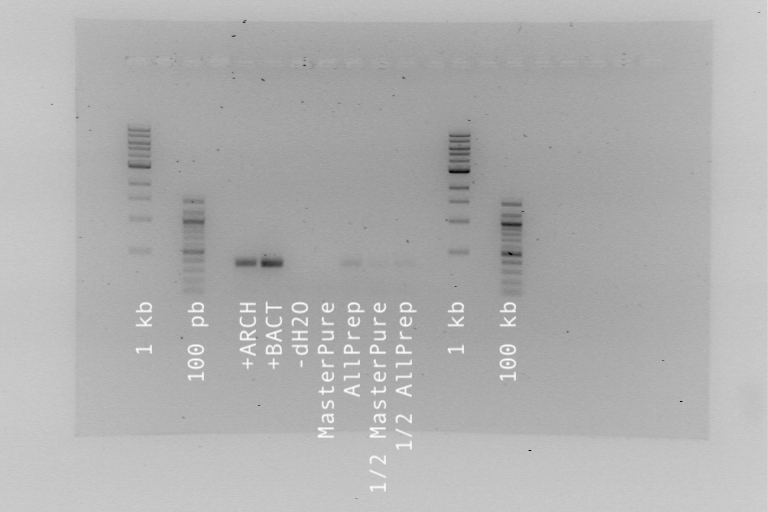
\includegraphics[width=\textwidth]{graphics/pic/20180208_EMP_OneTaq_kits_inverted.png}
\end{figure}
